\documentclass{sigchi}

% Use this section to set the ACM copyright statement (e.g. for
% preprints).  Consult the conference website for the camera-ready
% copyright statement.

% Copyright
\CopyrightYear{2016}
%\setcopyright{acmcopyright}
% \setcopyright{acmlicensed}
\setcopyright{rightsretained}
%\setcopyright{usgov}
%\setcopyright{usgovmixed}
%\setcopyright{cagov}
%\setcopyright{cagovmixed}
% DOI
\doi{N/A}
% ISBN
\isbn{N/A}
%Conference
% \conferenceinfo{CHI'16,}{May 07--12, 2016, San Jose, CA, USA}
%Price
% \acmPrice{\$15.00}

% Use this command to override the default ACM copyright statement
% (e.g. for preprints).  Consult the conference website for the
% camera-ready copyright statement.

%% HOW TO OVERRIDE THE DEFAULT COPYRIGHT STRIP --
%% Please note you need to make sure the copy for your specific
%% license is used here!
% \toappear{
% Permission to make digital or hard copies of all or part of this work
% for personal or classroom use is granted without fee provided that
% copies are not made or distributed for profit or commercial advantage
% and that copies bear this notice and the full citation on the first
% page. Copyrights for components of this work owned by others than ACM
% must be honored. Abstracting with credit is permitted. To copy
% otherwise, or republish, to post on servers or to redistribute to
% lists, requires prior specific permission and/or a fee. Request
% permissions from \href{mailto:Permissions@acm.org}{Permissions@acm.org}. \\
% \emph{CHI '16},  May 07--12, 2016, San Jose, CA, USA \\
% ACM xxx-x-xxxx-xxxx-x/xx/xx\ldots \$15.00 \\
% DOI: \url{http://dx.doi.org/xx.xxxx/xxxxxxx.xxxxxxx}
% }

% Arabic page numbers for submission.  Remove this line to eliminate
% page numbers for the camera ready copy
% \pagenumbering{arabic}

% Load basic packages
\usepackage{balance}       % to better equalize the last page
\usepackage{graphics}      % for EPS, load graphicx instead
\usepackage[T1]{fontenc}   % for umlauts and other diaeresis
\usepackage{txfonts}
\usepackage{mathptmx}
\usepackage[pdflang={en-US},pdftex]{hyperref}
\usepackage{color}
\usepackage{booktabs}
\usepackage{textcomp}

% Some optional stuff you might like/need.
\usepackage{microtype}        % Improved Tracking and Kerning
% \usepackage[all]{hypcap}    % Fixes bug in hyperref caption linking
\usepackage{ccicons}          % Cite your images correctly!
% \usepackage[utf8]{inputenc} % for a UTF8 editor only

% If you want to use todo notes, marginpars etc. during creation of
% your draft document, you have to enable the "chi_draft" option for
% the document class. To do this, change the very first line to:
% "\documentclass[chi_draft]{sigchi}". You can then place todo notes
% by using the "\todo{...}"  command. Make sure to disable the draft
% option again before submitting your final document.
\usepackage{todonotes}

% Paper metadata (use plain text, for PDF inclusion and later
% re-using, if desired).  Use \emtpyauthor when submitting for review
% so you remain anonymous.
\def\plaintitle{Predicting Asthmatic Events from Environmental Variables}
\def\plainauthor{Yuriy Minin}
\def\emptyauthor{}
\def\plainkeywords{asthma; dust sensors; personal informatics; personal data; health tracking;}

% llt: Define a global style for URLs, rather that the default one
\makeatletter
\def\url@leostyle{%
  \@ifundefined{selectfont}{
    \def\UrlFont{\sf}
  }{
    \def\UrlFont{\small\bf\ttfamily}
  }}
\makeatother
\urlstyle{leo}

% To make various LaTeX processors do the right thing with page size.
\def\pprw{8.5in}
\def\pprh{11in}
\special{papersize=\pprw,\pprh}
\setlength{\paperwidth}{\pprw}
\setlength{\paperheight}{\pprh}
\setlength{\pdfpagewidth}{\pprw}
\setlength{\pdfpageheight}{\pprh}

% Make sure hyperref comes last of your loaded packages, to give it a
% fighting chance of not being over-written, since its job is to
% redefine many LaTeX commands.
\definecolor{linkColor}{RGB}{6,125,233}
\hypersetup{%
  pdftitle={\plaintitle},
  pdfauthor={\plainauthor},
  pdfkeywords={\plainkeywords},
  pdfdisplaydoctitle=true, % For Accessibility
  bookmarksnumbered,
  pdfstartview={FitH},
  colorlinks,
  citecolor=black,
  filecolor=black,
  linkcolor=black,
  urlcolor=linkColor,
  breaklinks=true,
  hypertexnames=false
}

% create a shortcut to typeset table headings
% \newcommand\tabhead[1]{\small\textbf{#1}}

% End of preamble. Here it comes the document.
\begin{document}

\title{\plaintitle}

\numberofauthors{1}
\author{%
  \alignauthor{Yuriy Minin\\
    \affaddr{Personal Informatics - INF350E}\\
    \affaddr{Austin, USA}\\
    \email{yuriym@utexas.edu}}\\
}

\maketitle

\begin{abstract}
  This report documents the results of a proof of concept study on a process for
  gathering personal air quality data for the purpose of predicting asthmatic
  events. The system gathers air particulate data through a laser based dust
  sensor module. This data was then analyzed in order to create a heat map for
  the areas around my daily route that provide the most risk for asthma related
  incidents. Existing solutions are either extremely expensive or are too bulky
  and unwieldy for daily usage. The device concept presented in this report can
  be dramatically reduced in size with the use of specialized hardware. Rapid
  prototyping technologies such as Arduino and Grove were used in in the
  development of this device in order to reduce the time requirements. Future
  work involes further reducing the device size and integrating with commonplace
  personal computer devices such as smartphones.
\end{abstract}

\category{H.5.m.}{Information Interfaces and Presentation
  (e.g. HCI)}{Miscellaneous}{}{}

\keywords{\plainkeywords}

\section{Introduction}

Asthma can sometimes be a life threatening condition, and yet can still appear
seemingly at random. It would be invaluable to be able to see ahead of time
what areas I am most prone to asthmatic events and when I am in danger. This
could also be easily extended to other individuals with the same condition who
could be regularly traveling in the same areas, very likely on a college campus.

Measurement of lung function through spirometry is currently the most accurate
method of predicting asthmatic risk. This form of measurment is typically
conducted in a clinical setting, not in the daily environment of the patient.
In addition this method is invasive and impractical for daily feedback routines.
As such, I focus on the development of a non-invasive passive system based on
environmental factors that can be used to predict asthmatic risk and inflammation.
Common environmental factors in asthmatic risk are air pollutants. Two key air
pollutants can affect asthma. One is ozone (found in smog). The other is
particle pollution (found in haze, smoke, and dust). When ozone and particle
pollution are in the air, adults and children with asthma are more likely to
have symptoms. \cite{asthma:flyer}

Development of a personal logging device in order to constantly monitor air
particulate data and ozone would help to provide a feedback system whereby I am
able to visualize what areas in my daily routine place me the most at risk for
asthmatic exacerbations.

Beyond respiratory diseases, the continuous monitoring of health and environment
through wearable devices has the potential to create a paradigm shift in
improving healthcare by empowering patients and doctors to transition from
managing illness to managing wellness and outcomes.

\section{Prior Work}
Much of the previous work has been based on tracking geolocation data of when a
user has to actively use their inhaler such as with the CareTRx "smart inhaler"
\url{https://www.caretrx.com/} This solution keeps a record of the all of the
user's asthmatic events recordedin a cloud based server system. \cite{caretrx} However, this
leaves out the entirety of a lower class of events called asthmatic exacerbations. During these
events, a patient suffering from asthma can feel the onset of asthma related
symptoms such as tightness of airways and wheezing of the lungs, however they
not temporarily disabled as with an asthma attack.

There are many studies showing the correlation between environmental factors and
an increase in asthmatic exacerbations. \cite{farr_2016, weber} They provide an
excellent base for a predictive model of asthmatic occurances.

Finally, there is a wearable device that attempts to accomplish the same goal as
this project. The HET system from NC State University uses local temperature
and humidity data along with data related to the wheezing of the user's lungs
in order to predict when they are in danger of an asthma attack.
This system does not keep a record of previous asthmatic events, and in
addition it is extremely intrusive and bulky. \cite{lowpower} This project does
a very good job at predicting when a patient is at risk for an asthma attack but
does not provide any way for them to aggregate and visualize their own personal
data.

I believe I can design a system that is more natural to use and accomplishes
the same results using a mobile application and a "clip on" base station that
would attach to a backpack or other personal item. This would accomplish many of
the results of previous solutions, while still remaining a passive sensing
technology.


\section{Implementation}

To serve as a proof of concept and to develop the area of personal logging
devices. I have developed a small integrated sensor and controller module that
logs dust particulate data around the wearer at all times. There are 2 primary
components of the sensor platform.

\begin{itemize}
\item A Grove Shinyei PPD42NS dust sensor (Figure 1).
\item Arduino Uno Microcontroller.
\end{itemize}

This sensor module then communicates with a python application running on a
personal laptop computer contained within my backpack. The main purpose of the
laptop computer is for integrating a geolocation tag with every sensor
measurement. Ideally, there would be integration with a smartphone device in order
to acquire GPS coordinates, however there were design limitations that will be
discussed in a later section.

\subsection{Dust Sensor}

This was an off the shelf Grove compatible component that allowed me the rapidly
prototype a module that could reliably measure air particulate data. This Dust
Sensor measures the Particulate Matter level in air by counting the Lo Pulse Occupancy
time(LPO time) in given time unit. LPO time is in proportion to PM concentration.
This sensor can provide pretty reliable data for air purifier system because
it's still responsive to particulates whose diameter is \( 1\ \mu \)m

\begin{figure}
\centering
  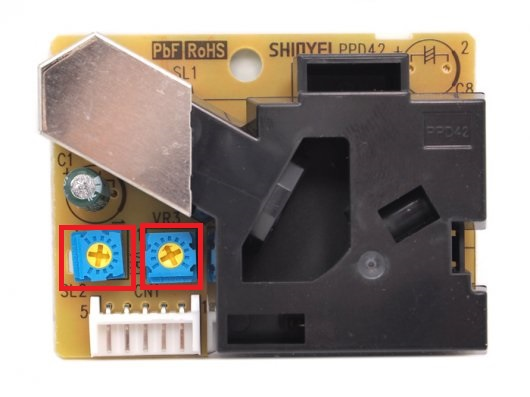
\includegraphics[width=1\columnwidth]{figures/sensor}
  \caption{ Shinyei PPD42NS dust sensor }~\label{fig:figure1}
\end{figure}

\begin{figure}
\centering
  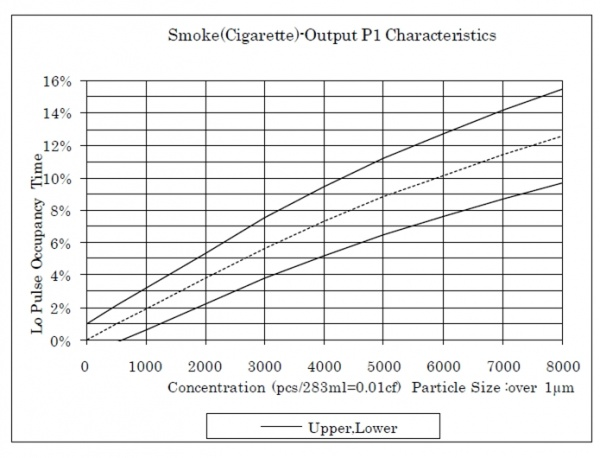
\includegraphics[width=1\columnwidth]{figures/characteristics}
  \caption{ Shinyei PPD42NS dust sensor chacteristic graph}~\label{fig:figure2}
\end{figure}

It is possible to calculate a concentration of particulate by looking
at the characteristic graph of the sensor. (Figure 2) By fitting a cubic polynomial
to this charactertic graph, we can calulate the particulate density from the LPO.

When using this in the Arduino sketch we can implement as:

\begin{verbatim}
  ratio = lowpulseoccupancy/(sampletime_ms*10.0);
  concentration = 1.1*pow(ratio,3)-3.8*pow(ratio,2)
    +520*ratio+0.62;
\end{verbatim}

This possible on the the Arduino because of the high sampling rate of the
digital pins on the system. A limitation that I found on the Raspberry Pi system
was that the GPIO header was unable to sample at the frequencies used by the LPO
output of the sensor module.

\subsection{Arduino Integration}

In integrating the sensor with the Arduino, I was required to use pin D8
on the ATmega328P board architecture. The sampling functionality could only be accomplished
by this SMD based analog pin.

The Shinyei PPD42NS dust sensor was wired to the Arduino Uno board as follows:

\begin{verbatim}
  JST Pin 1 => Arduino GND
  JST Pin 3 => Arduino 5VDC
  JST Pin 4 => Arduino Digital Pin 8
\end{verbatim}

The Arduino was powered by a personal laptop computer that was near the device at
all times. This was an unfortunate limitation due to power requirements and need
to integrate location data with the sensor readings

\section{Study and Discussion}

The device was worn by me for a period of about 8 hours during the most active
part of my day. I attached the sensor to my shoulder and my laptop and started
the python based logging application that I wrote in order to gather the data
from the sensor and then append a geolocation tag to each one. The geolocation
was acquired through a MacOS based script written by Rob Mathers. \cite{whereami}
The script returned a latitude and longitude based on WPS coordinates optained from
the MacOS CoreLocation API. Preliminary testing on this data proved that it was
extremely accurate in determining my current location whenever I was connected to
WiFi. A location is obtained by measuring the intensity of the received signal from
any wireless access points within range of my computer and then comparing these
to a public hotspot database that is developed from mobile device GPS location data. \cite{zahradnik}

\begin{figure}
\centering
  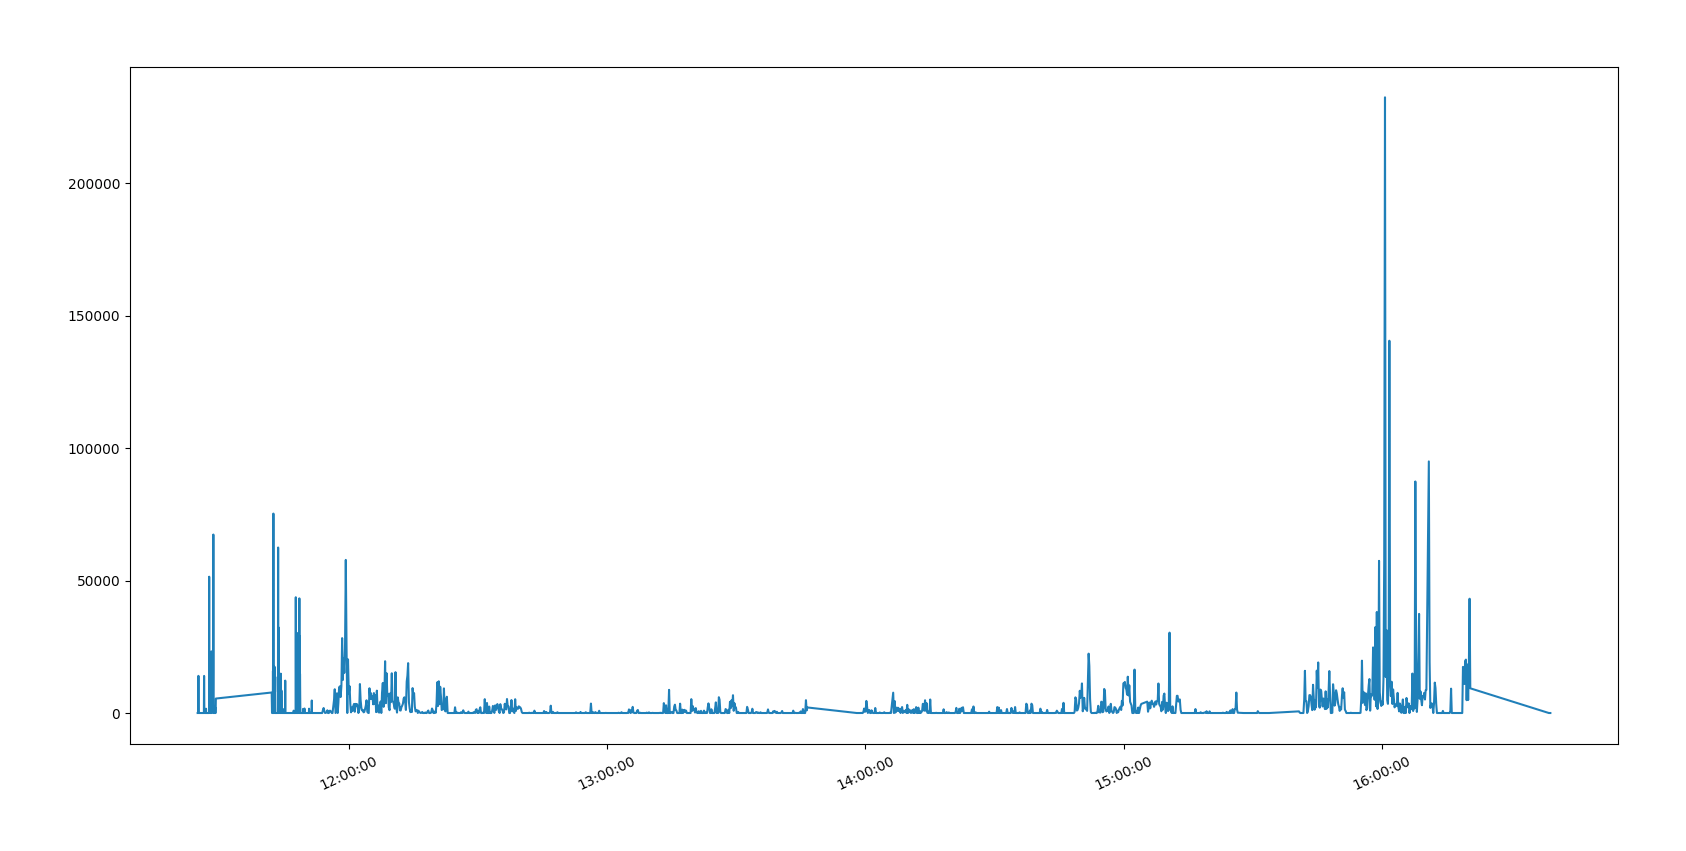
\includegraphics[width=1\columnwidth]{figures/concentration}
  \caption{ Concentration of particulate matter around me throughout my 8 hour workday.
  }~\label{fig:figure3}
\end{figure}

After the 8 hour logging period, a measurment of a time series representation of
the particulate concentration in my daily routine was obtained. This can be seen in Figure 3.
Looking at this graph, we can see a few period throughout the day where the air quality around
me deteriorated dramatically. Those are when I left the indoor office where I do
most of my daily work to go eat with friends or walk across campus for a class.
There are also a few timeskips. In the first part of the data series, my laptop
ran out of battery so there was period of about 15 minutes where I was unable to collect data.
In addition, just after 14:00 someone needed to borrow the cable that I was using
to monitor serial data from my Arduino in order to print something froma shared
printing station. An unfortunate side effect of using shared equipment.
The spikes at the beginning and end of the series are when I was walking near construction
on Speedway. The dust clouds from the loose earth provided a great opportunity to compare
indoor and outdoor air quality during my time wearing the sensor.

In Figure 4, we can see a map of the area surrounding my daily route with annotated pins
marking the particulate measurements that I took throughout the day. This is the most
useful graphic for personal reflection that I have generated. On the graph, all points
are colorized according to these divisions. \cite{mapper}

\begin{itemize}
\item 0-1000: Green
\item 1000-5000: Yellow
\item <5000: Red
\end{itemize}

From this chart, I can glean which areas
around campus are the most dangerous for me in terms of the impact that they can have on
my asthma.

Unfortunately, the most dangerous areas were those just outside the IEEE student
offices which is where I spend most of my free time on campus working on class work.
It will be difficult for me to find a way to practically avoid those areas. But it
still provides an interesting proof on concept on analyzing location based heat maps
of asthmatic risk.

There are also some inaccuracies in the methods that I used to gather data. When
collecting my data I was using the particulate sensor with the main detection area
completely open to sunlight. While the sensor is designed to detect the wavelengths
of the laser specifically, this may have contaminated a portion of my data. Repetition
and additional data collection will be necessary in order to rule that out as a
possibility.

\begin{figure}
\centering
  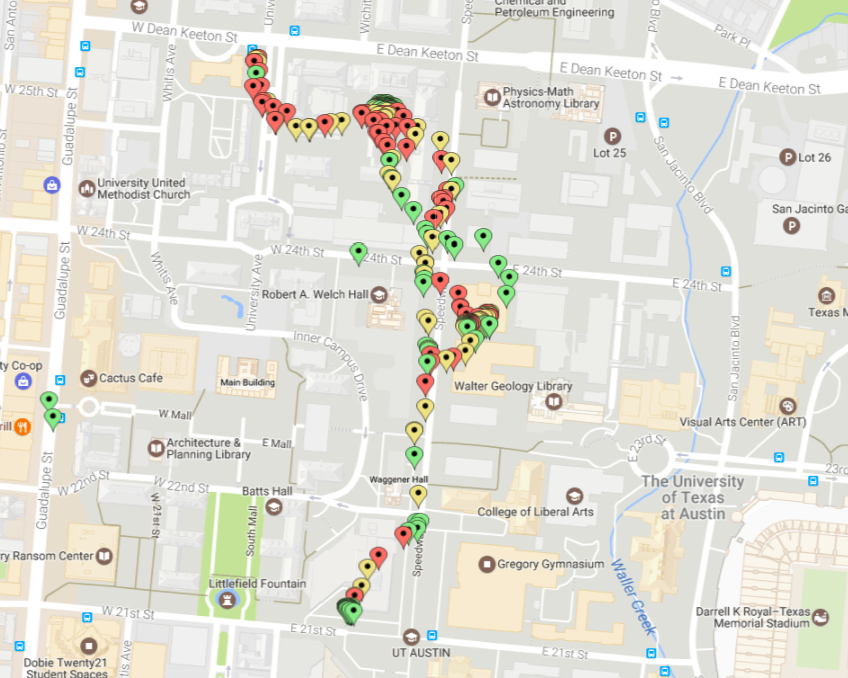
\includegraphics[width=0.9\columnwidth]{figures/map}
  \caption{ Aggregation of all the geolocation tags with particle concentrations
  mapped to differnt colors of pins.
  }~\label{fig:figure4}
\end{figure}

\section{Contributions}

All of the data acquired during this study was collected by myself over a single day.
The device was built over a period of 2 weeks after having quite a bit of trouble
integrating the sensor module into various platforms. Unlike previous efforts to develop
an asthma prediction system. This one focuses on using continuous personal data
and self reflection in order to develop change in personal habit. This is unique from
previous studies in this area, which focus on predictive modeling. \cite{lowpower, farr_2016}

All the code written for this assignment can be found at https://github.com/yursky/asthma-prediction.


\section{Future Work}

This project presents many different areas that I hope I can expand on in the future.
One of the greatest hardware limitations that I struggled with throughout this project
was serial communications from the Arduino microcontrollers. In my mind, the ideal
module structure would be a standalone sensor, Arduino, and battery combination that
I could keep connected via Bluetooth to my smartphone. I would then be free to use the
GPS capabilities of the mobile device and keep the sensor module very portable. This small
change would drastically improve the ease of carrying the sensor around.

In addition, the aggregation of asthmatic events that I encounter through a smart
inhaler, similar to many products currently available, would allow me to create a
personalized predictive model of what environmental conditions trigger my asthma.
This would provide valuable insights to any patient who suffers from asthma.
By slightly altering your day to day behavior (e.g taking a different route to class)
an individual would be able to lower the risk of a dangerous asthma attack.

Once the sensor is integrated with a smarthphone, a complete suite of monitoring
and insight tools can be developed to simplify respiratory disease management. a
web based dashboard similar to CareTRx's could be developed that aggregates and
visualizes the patient's personalized profile of particulate data. \cite{caretrx}
This also provides the opportunity to explore various areas of user design and
visualization in the interface developed for the mobile device. 

\section{Conclusions}

Low power and low cost portable devices for monitoring air particulates can be developed
to aid individuals with managing asthma and other chronic respiratory diseases.
These devices can provide extremely valuable insights to users about information
related to their personal behaviors and the eventual consequences that they lead to.

This area has a lot of exciting potential for future developments especially in my
own designs. I hope to be able to continue working on this in the near future.




% Balancing columns in a ref list is a bit of a pain because you
% either use a hack like flushend or balance, or manually insert
% a column break.  http://www.tex.ac.uk/cgi-bin/texfaq2html?label=balance
% multicols doesn't work because we're already in two-column mode,
% and flushend isn't awesome, so I choose balance.  See this
% for more info: http://cs.brown.edu/system/software/latex/doc/balance.pdf
%
% Note that in a perfect world balance wants to be in the first
% column of the last page.
%
% If balance doesn't work for you, you can remove that and
% hard-code a column break into the bbl file right before you
% submit:
%
% http://stackoverflow.com/questions/2149854/how-to-manually-equalize-columns-
% in-an-ieee-paper-if-using-bibtex
%
% Or, just remove \balance and give up on balancing the last page.
%

% BALANCE COLUMNS
\balance{}

% REFERENCES FORMAT
% References must be the same font size as other body text.
\bibliographystyle{SIGCHI-Reference-Format}
\bibliography{sample}

\end{document}

%%% Local Variables:
%%% mode: latex
%%% TeX-master: t
%%% End:
